\chapter{Supplementary Internal Evaluation}
\label{apendice:internal-evaluation}

\section{Training Convergence Across Runs}
\label{sec:appendix-training-details}

This section provides the complete convergence documentation for the six deterministic training runs. The figures and tables below document per-run checkpoint selection and did not, by themselves, determine the final external-evaluation candidate.

\FloatBarrier
% Generated by scripts/publish_workflow_results_to_thesis.py. Do not edit.
\begingroup
\setlength{\intextsep}{4pt}
\begin{figure}[htbp]
\centering
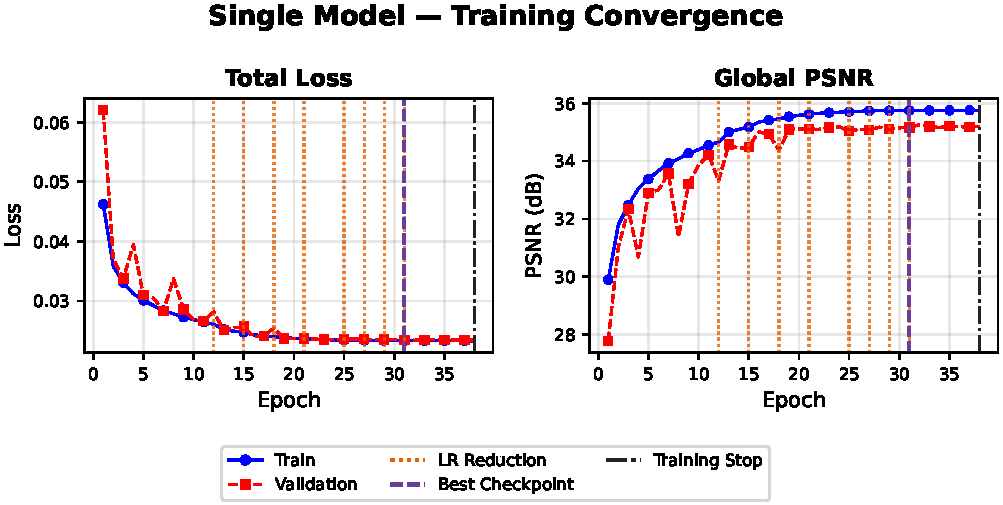
\includegraphics[width=0.98\linewidth]{Figures/Generated/training/training-curves-singlehead-pair-01-loss-psnr-2dbea9f5.pdf}
\end{figure}

\begin{figure}[htbp]
\centering
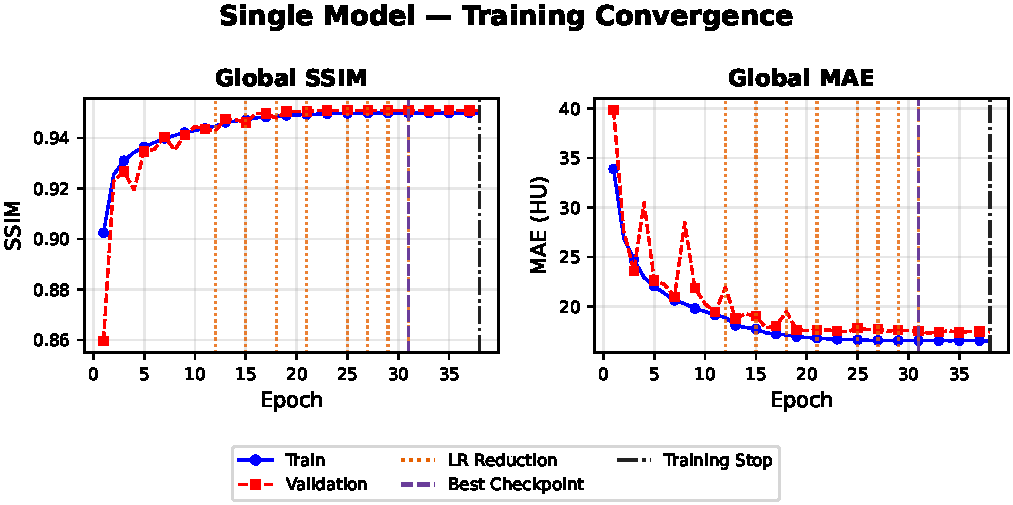
\includegraphics[width=0.98\linewidth]{Figures/Generated/training/training-curves-singlehead-pair-02-ssim-mae-c7bfb6d4.pdf}
\end{figure}

\begin{figure}[htbp]
\centering
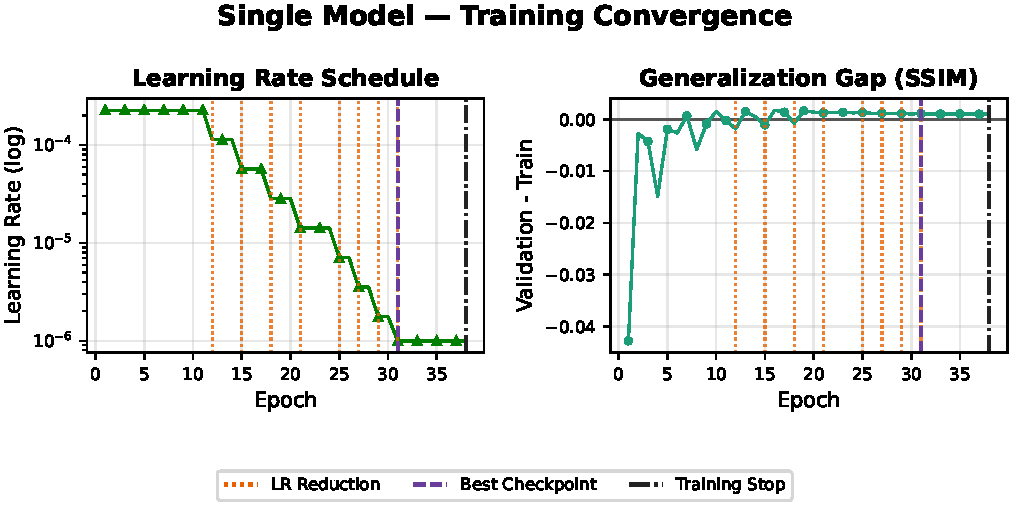
\includegraphics[width=0.98\linewidth]{Figures/Generated/training/training-curves-singlehead-pair-03-lr-gap-be217cb8.pdf}
\end{figure}

\FloatBarrier
\captionsetup{skip=1.5pt}
\graphiccaptionof[Training convergence: Single Model, seed 42]{Training convergence for the Single Model, seed 42. Each chart pair repeats the shared legend so it remains interpretable if the group spans multiple pages. Orange dotted vertical lines indicate learning-rate reductions; the purple dashed line marks the epoch of the best validation checkpoint; and the black dash-dotted line marks training termination. The \textit{generalization-gap} panel reports validation minus training SSIM and supports inspection for persistent divergence compatible with overfitting.}
\label{fig:appendix-training-convergence-single-model-seed-42}
\par\medskip
\endgroup

\begingroup
\setlength{\intextsep}{4pt}
\begin{figure}[htbp]
\centering
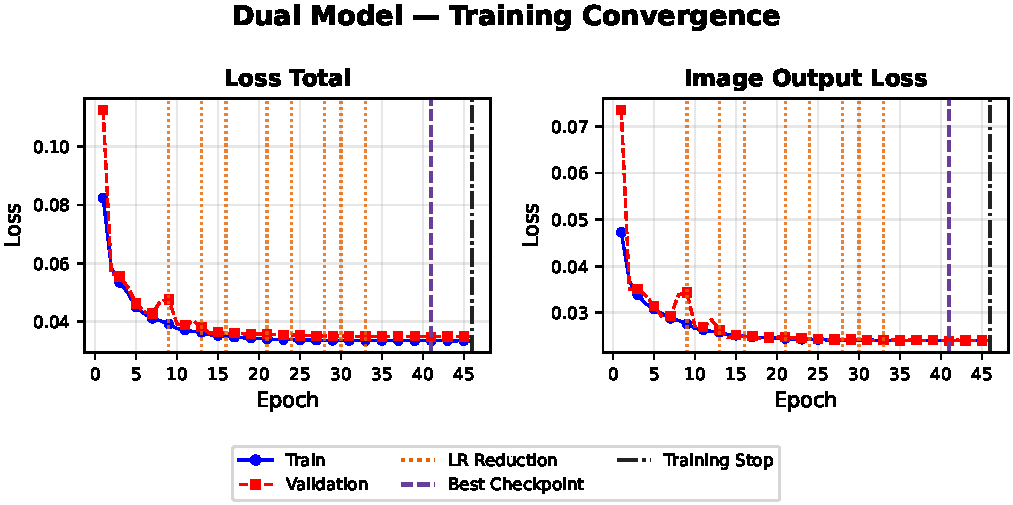
\includegraphics[width=0.98\linewidth]{Figures/Generated/training/training-curves-dualhead-pair-01-loss-e3314fde.pdf}
\end{figure}

\begin{figure}[htbp]
\centering
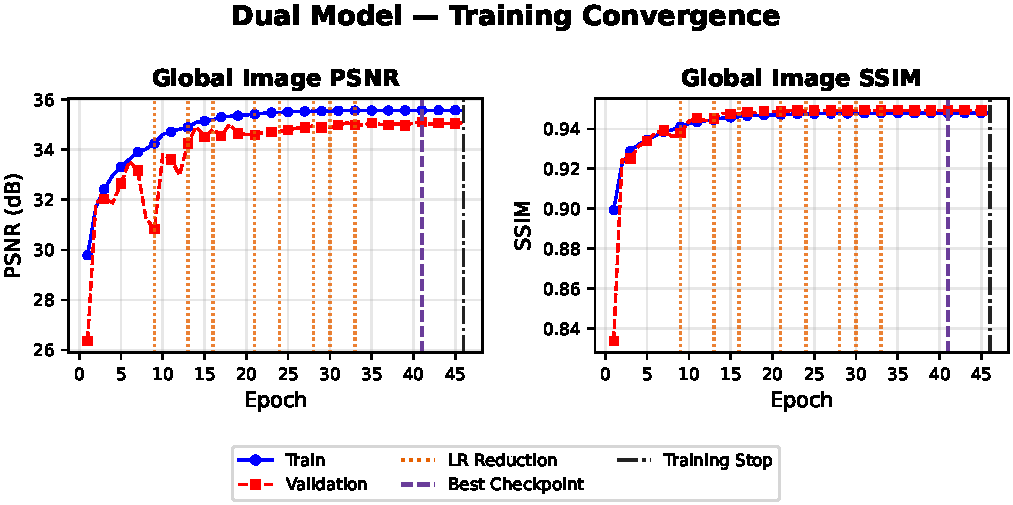
\includegraphics[width=0.98\linewidth]{Figures/Generated/training/training-curves-dualhead-pair-02-psnr-ssim-edde567e.pdf}
\end{figure}

\begin{figure}[htbp]
\centering
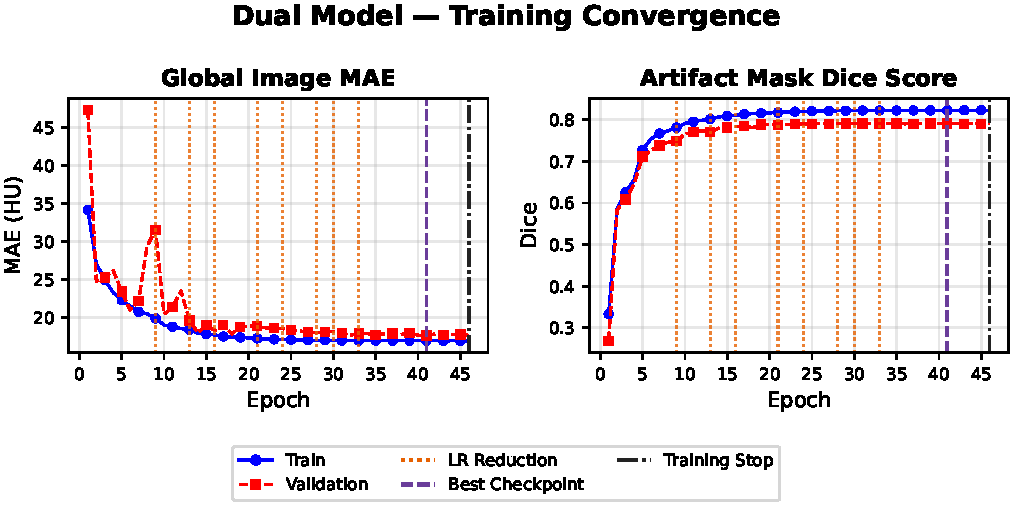
\includegraphics[width=0.98\linewidth]{Figures/Generated/training/training-curves-dualhead-pair-03-mae-dice-16a94110.pdf}
\end{figure}

\begin{figure}[htbp]
\centering
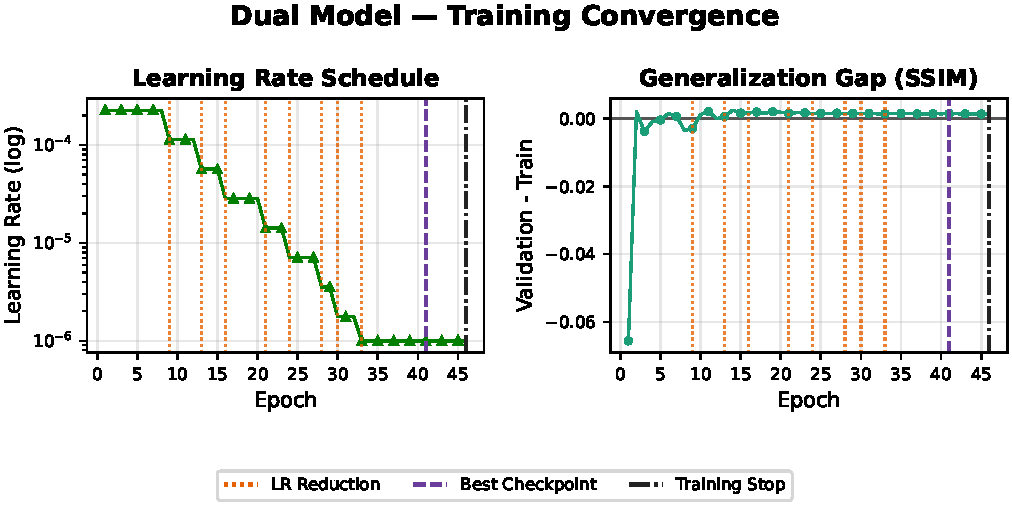
\includegraphics[width=0.98\linewidth]{Figures/Generated/training/training-curves-dualhead-pair-04-lr-gap-f902b5f6.pdf}
\end{figure}

\FloatBarrier
\captionsetup{skip=1.5pt}
\graphiccaptionof[Training convergence: Dual Model, seed 42]{Training convergence for the Dual Model, seed 42. Each chart pair repeats the shared legend so it remains interpretable if the group spans multiple pages. Orange dotted vertical lines indicate learning-rate reductions; the purple dashed line marks the epoch of the best validation checkpoint; and the black dash-dotted line marks training termination. The \textit{generalization-gap} panel reports validation minus training SSIM and supports inspection for persistent divergence compatible with overfitting.}
\label{fig:appendix-training-convergence-dual-model-seed-42}
\par\medskip
\endgroup

\begingroup
\setlength{\intextsep}{4pt}
\begin{figure}[htbp]
\centering
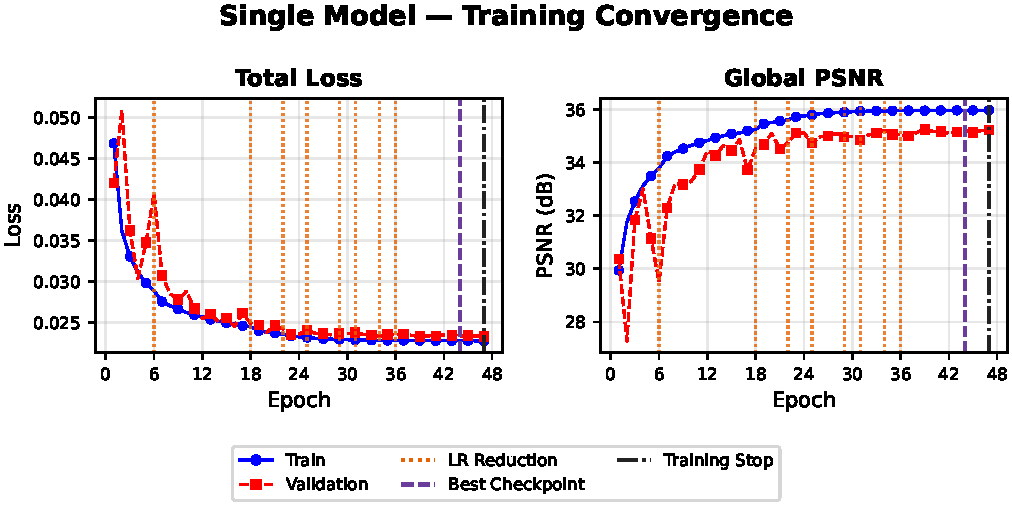
\includegraphics[width=0.98\linewidth]{Figures/Generated/training/training-curves-singlehead-pair-01-loss-psnr-2b6ea850.pdf}
\end{figure}

\begin{figure}[htbp]
\centering
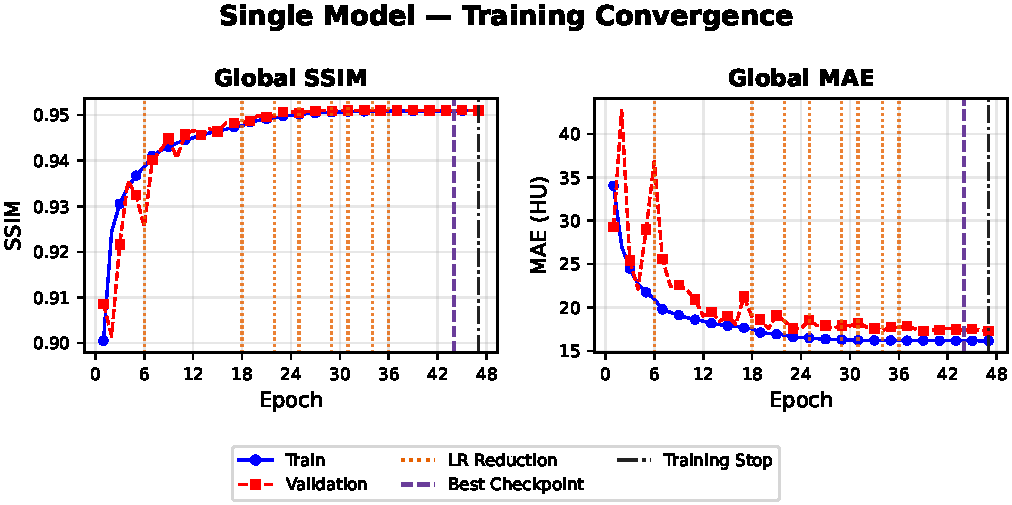
\includegraphics[width=0.98\linewidth]{Figures/Generated/training/training-curves-singlehead-pair-02-ssim-mae-dbf1eb22.pdf}
\end{figure}

\begin{figure}[htbp]
\centering
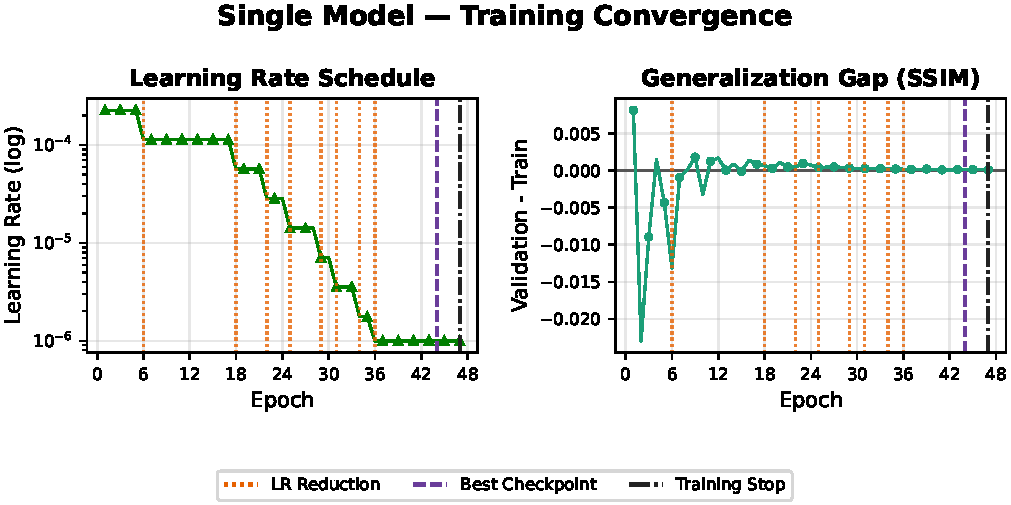
\includegraphics[width=0.98\linewidth]{Figures/Generated/training/training-curves-singlehead-pair-03-lr-gap-31221acf.pdf}
\end{figure}

\FloatBarrier
\captionsetup{skip=1.5pt}
\graphiccaptionof[Training convergence: Single Model, seed 1337]{Training convergence for the Single Model, seed 1337. Each chart pair repeats the shared legend so it remains interpretable if the group spans multiple pages. Orange dotted vertical lines indicate learning-rate reductions; the purple dashed line marks the epoch of the best validation checkpoint; and the black dash-dotted line marks training termination. The \textit{generalization-gap} panel reports validation minus training SSIM and supports inspection for persistent divergence compatible with overfitting.}
\label{fig:appendix-training-convergence-single-model-seed-1337}
\par\medskip
\endgroup

\begingroup
\setlength{\intextsep}{4pt}
\begin{figure}[htbp]
\centering
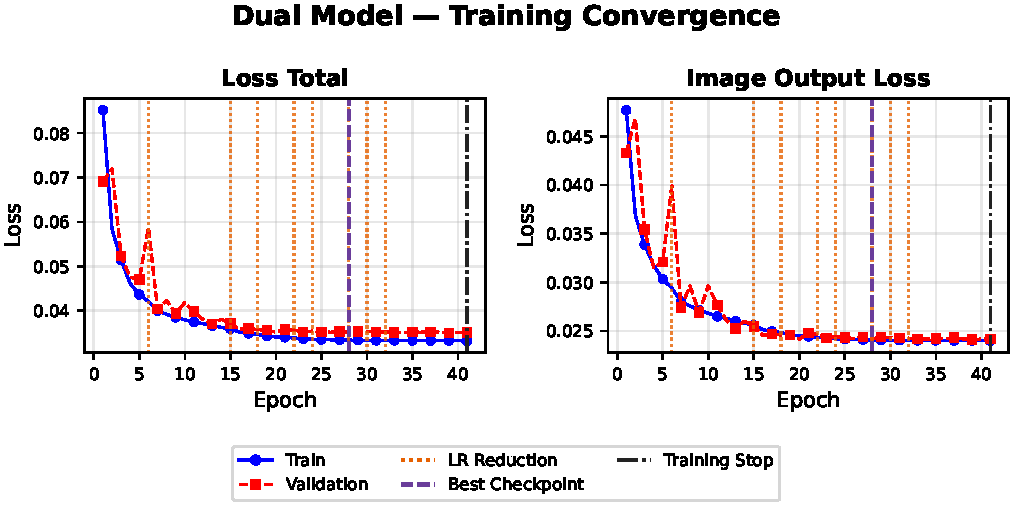
\includegraphics[width=0.98\linewidth]{Figures/Generated/training/training-curves-dualhead-pair-01-loss-ad3e34d5.pdf}
\end{figure}

\begin{figure}[htbp]
\centering
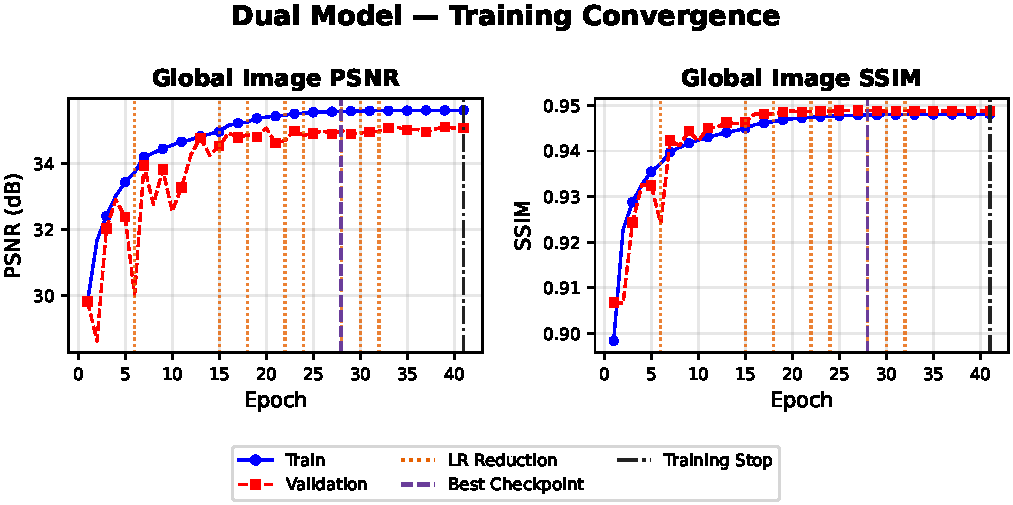
\includegraphics[width=0.98\linewidth]{Figures/Generated/training/training-curves-dualhead-pair-02-psnr-ssim-a2bedecb.pdf}
\end{figure}

\begin{figure}[htbp]
\centering
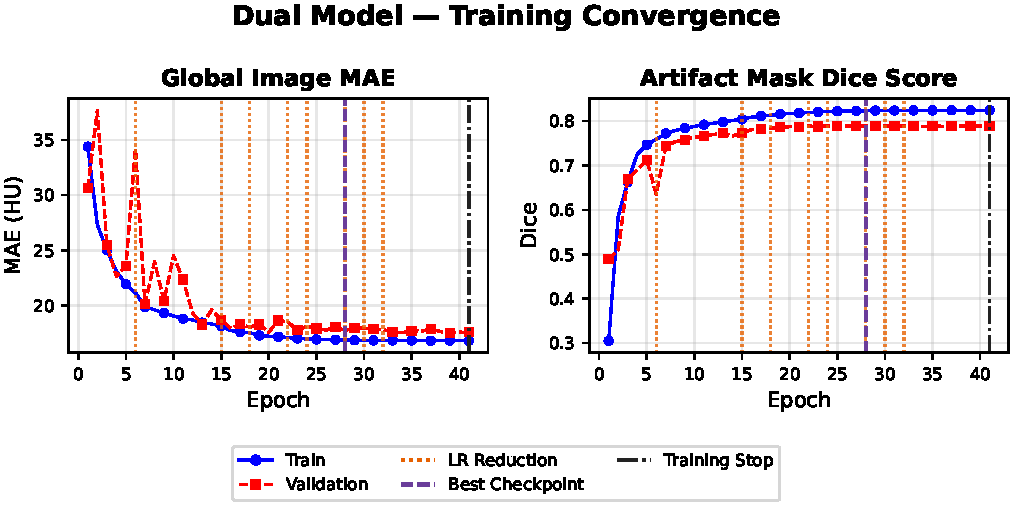
\includegraphics[width=0.98\linewidth]{Figures/Generated/training/training-curves-dualhead-pair-03-mae-dice-3c0cd1ca.pdf}
\end{figure}

\begin{figure}[htbp]
\centering
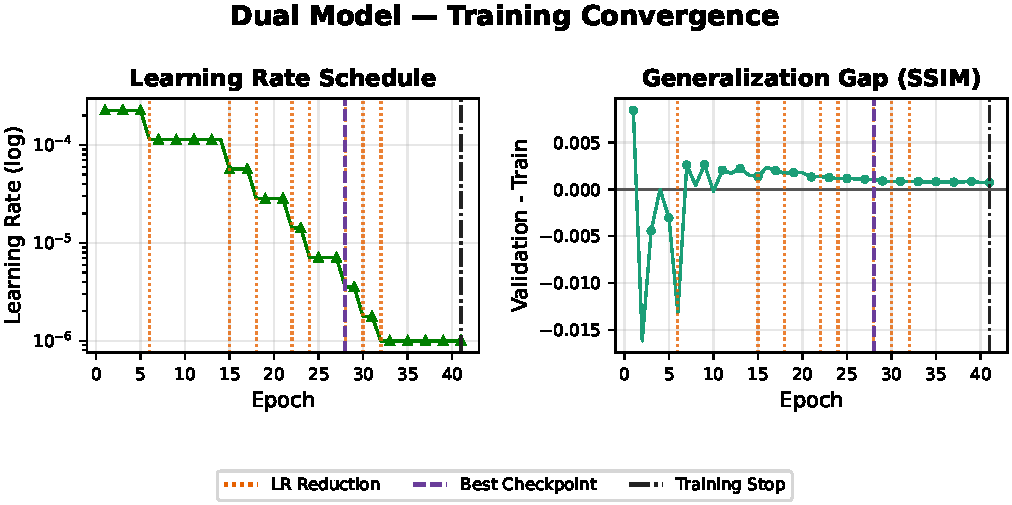
\includegraphics[width=0.98\linewidth]{Figures/Generated/training/training-curves-dualhead-pair-04-lr-gap-3f97ba9f.pdf}
\end{figure}

\FloatBarrier
\captionsetup{skip=1.5pt}
\graphiccaptionof[Training convergence: Dual Model, seed 1337]{Training convergence for the Dual Model, seed 1337. Each chart pair repeats the shared legend so it remains interpretable if the group spans multiple pages. Orange dotted vertical lines indicate learning-rate reductions; the purple dashed line marks the epoch of the best validation checkpoint; and the black dash-dotted line marks training termination. The \textit{generalization-gap} panel reports validation minus training SSIM and supports inspection for persistent divergence compatible with overfitting.}
\label{fig:appendix-training-convergence-dual-model-seed-1337}
\par\medskip
\endgroup

\begingroup
\setlength{\intextsep}{4pt}
\begin{figure}[htbp]
\centering
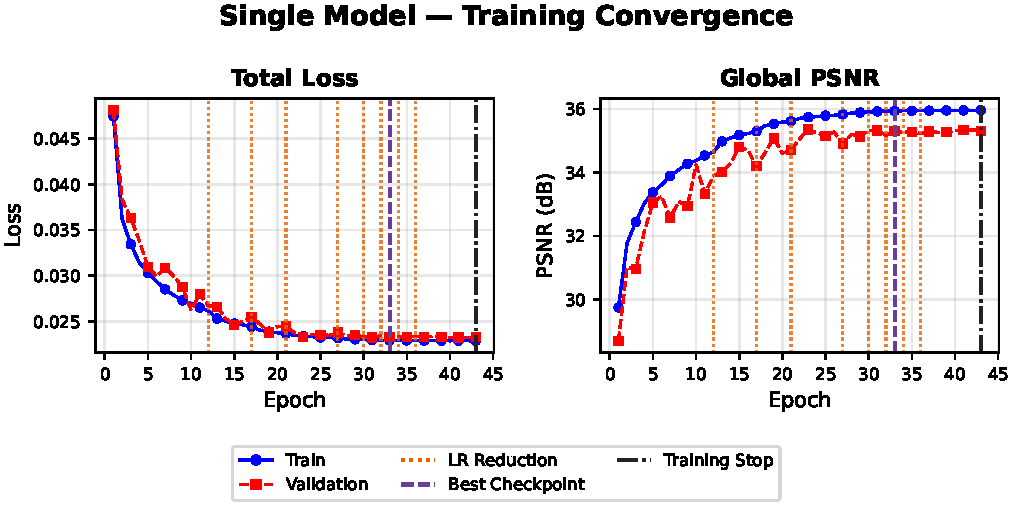
\includegraphics[width=0.98\linewidth]{Figures/Generated/training/training-curves-singlehead-pair-01-loss-psnr-6e359ebd.pdf}
\end{figure}

\begin{figure}[htbp]
\centering
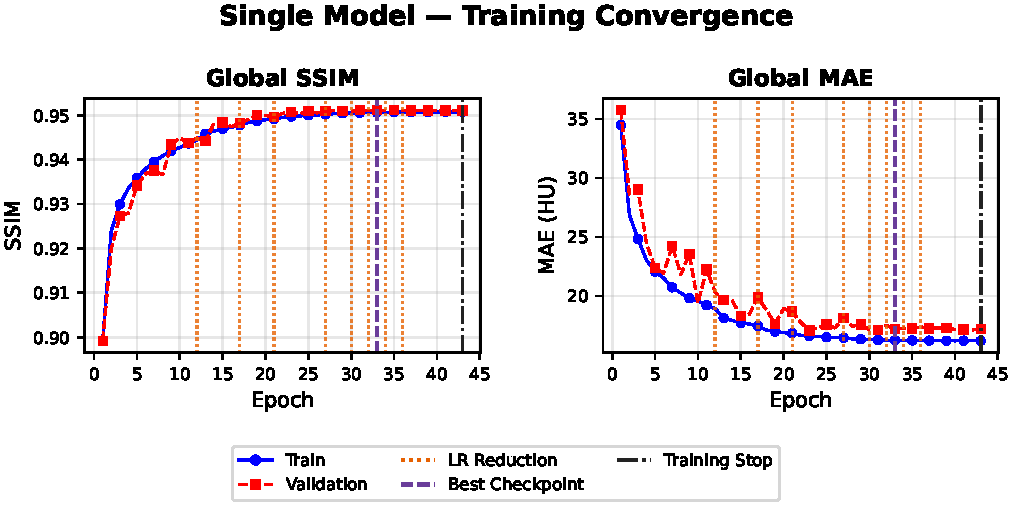
\includegraphics[width=0.98\linewidth]{Figures/Generated/training/training-curves-singlehead-pair-02-ssim-mae-80362d3f.pdf}
\end{figure}

\begin{figure}[htbp]
\centering
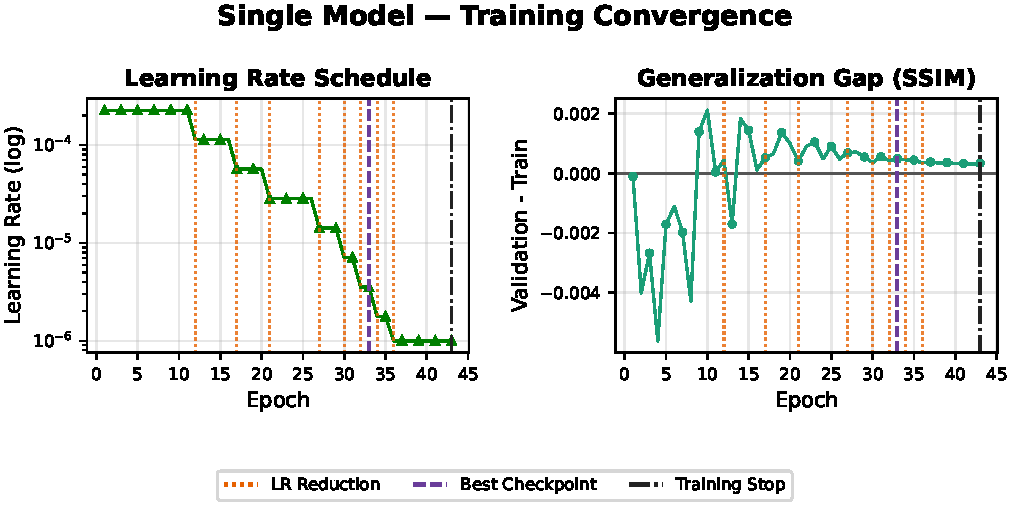
\includegraphics[width=0.98\linewidth]{Figures/Generated/training/training-curves-singlehead-pair-03-lr-gap-c975e425.pdf}
\end{figure}

\FloatBarrier
\captionsetup{skip=1.5pt}
\graphiccaptionof[Training convergence: Single Model, seed 2024]{Training convergence for the Single Model, seed 2024. Each chart pair repeats the shared legend so it remains interpretable if the group spans multiple pages. Orange dotted vertical lines indicate learning-rate reductions; the purple dashed line marks the epoch of the best validation checkpoint; and the black dash-dotted line marks training termination. The \textit{generalization-gap} panel reports validation minus training SSIM and supports inspection for persistent divergence compatible with overfitting.}
\label{fig:appendix-training-convergence-single-model-seed-2024}
\par\medskip
\endgroup

\begingroup
\setlength{\intextsep}{4pt}
\begin{figure}[htbp]
\centering
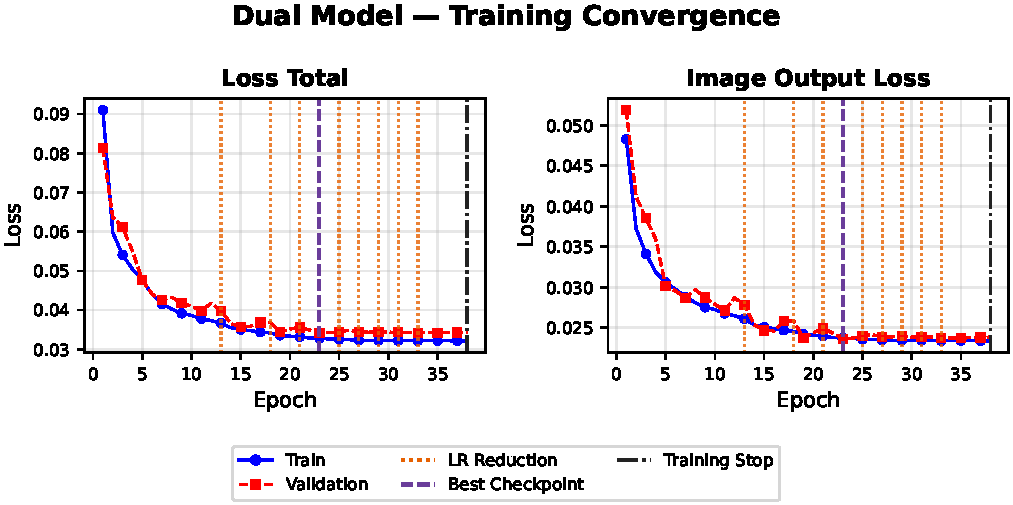
\includegraphics[width=0.98\linewidth]{Figures/Generated/training/training-curves-dualhead-pair-01-loss-419f6af3.pdf}
\end{figure}

\begin{figure}[htbp]
\centering
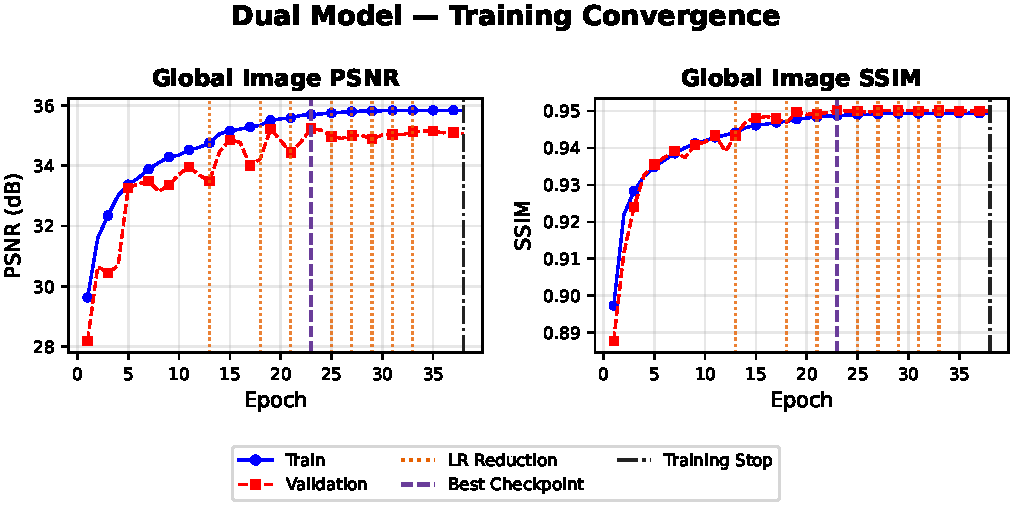
\includegraphics[width=0.98\linewidth]{Figures/Generated/training/training-curves-dualhead-pair-02-psnr-ssim-bc0a0156.pdf}
\end{figure}

\begin{figure}[htbp]
\centering
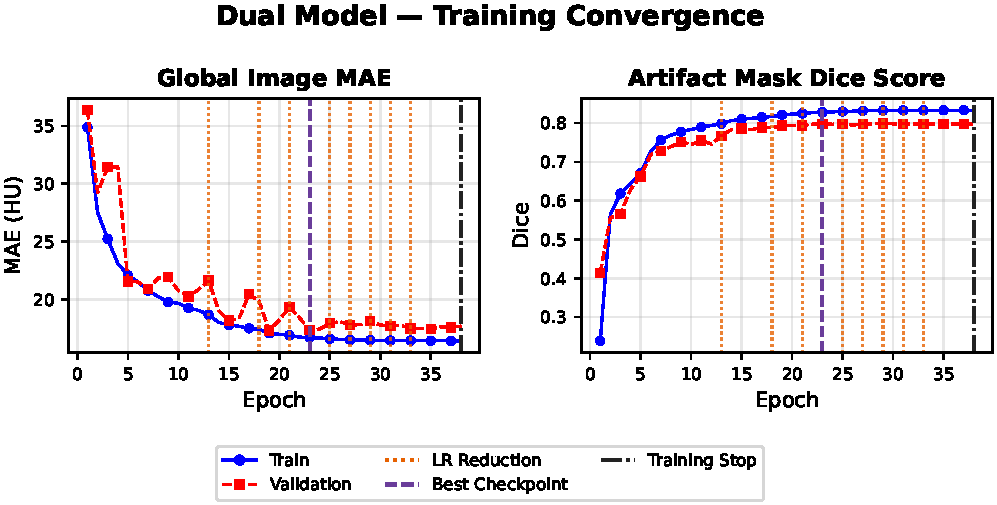
\includegraphics[width=0.98\linewidth]{Figures/Generated/training/training-curves-dualhead-pair-03-mae-dice-bde647ae.pdf}
\end{figure}

\begin{figure}[htbp]
\centering
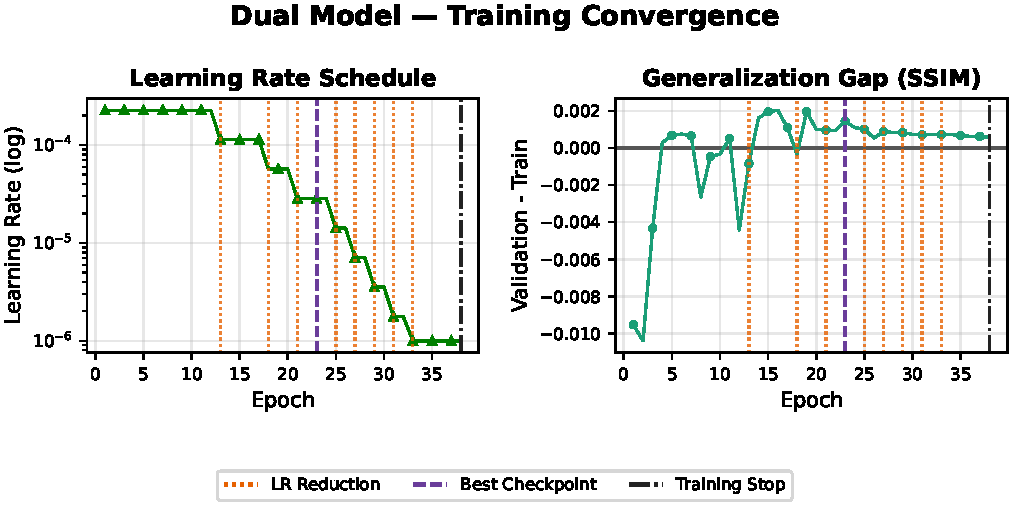
\includegraphics[width=0.98\linewidth]{Figures/Generated/training/training-curves-dualhead-pair-04-lr-gap-06e153c6.pdf}
\end{figure}

\FloatBarrier
\captionsetup{skip=1.5pt}
\graphiccaptionof[Training convergence: Dual Model, seed 2024]{Training convergence for the Dual Model, seed 2024. Each chart pair repeats the shared legend so it remains interpretable if the group spans multiple pages. Orange dotted vertical lines indicate learning-rate reductions; the purple dashed line marks the epoch of the best validation checkpoint; and the black dash-dotted line marks training termination. The \textit{generalization-gap} panel reports validation minus training SSIM and supports inspection for persistent divergence compatible with overfitting.}
\label{fig:appendix-training-convergence-dual-model-seed-2024}
\par\medskip
\endgroup


\FloatBarrier

% Best validation SSIM extracted from data/checkpoints/*/*/training_*.csv.
% For Dual Model, SSIM refers to the image-reconstruction output.
\begin{table}[!htbp]
\centering

\begin{tabular}{lccc}
\hline
 & \multicolumn{3}{c}{\textbf{Best SSIM (HU)}} \\
\hline
\textbf{Seed} & \textbf{42} & \textbf{1337} & \textbf{2024} \\
\hline
\textbf{Single Model} & 0.95096 (31)* & 0.95106 (44) & 0.95113 (33) \\
\textbf{Dual Model} & 0.94938 (41) & 0.94895 (28) & 0.95025 (23) \\
\hline
\end{tabular}
\par\smallskip
\footnotesize *Values in parentheses indicate the corresponding epoch.
\captionsetup{skip=2pt}
\caption[Best validation SSIM by model and seed]{Highest validation SSIM by model and seed, with the corresponding epoch. For the Dual Model, SSIM was calculated on the reconstructed-image output.}
\label{tab:best-validation-ssim}
\end{table}

% Validation PSNR at the epoch selected by the best validation SSIM.
% For Dual Model, both metrics refer to the image-reconstruction output.
\begin{table}[!htbp]
\centering

\begin{tabular}{lccc}
\hline
 & \multicolumn{3}{c}{\textbf{PSNR (dB) - Same Best SSIM Epoch }} \\
\hline
\textbf{Seed} & \textbf{42} & \textbf{1337} & \textbf{2024} \\
\hline
\textbf{Single Model} & 35.16365 (31) & 35.20020 (44) & 35.30099 (33) \\
\textbf{Dual Model} & 35.10422 (41) & 35.00705 (28) & 35.23622 (23) \\
\hline
\end{tabular}
\par\smallskip
\captionsetup{skip=2pt}
\caption[Validation PSNR at best validation SSIM]{Validation PSNR at the epoch selected by the highest validation SSIM, by model and seed. For the Dual Model, both metrics were calculated on the reconstructed-image output.}
\label{tab:best-validation-psnr}
\end{table}

% Validation MAE at the epoch selected by the best validation SSIM.
% For Dual Model, both metrics refer to the image-reconstruction output.
\begin{table}[!htbp]
\centering
\begin{tabular}{lccc}
\hline
 & \multicolumn{3}{c}{\textbf{MAE (HU) - Same Best SSIM Epoch}} \\
\hline
\textbf{Seed} & \textbf{42} & \textbf{1337} & \textbf{2024} \\
\hline
\textbf{Single Model} & 17.52002 (31) & 17.36296 (44) & 17.19180 (33) \\
\textbf{Dual Model} & 17.58006 (41) & 17.73584 (28) & 17.35387 (23) \\
\hline
\end{tabular}
\par\smallskip
\captionsetup{skip=2pt}
\caption[Validation MAE at best validation SSIM]{Validation MAE at the epoch selected by the highest validation SSIM, by model and seed. For the Dual Model, both metrics were calculated on the reconstructed-image output.}
\label{tab:mae-at-best-validation-ssim}
\end{table}

\FloatBarrier

This appendix presents complementary quantitative checks for the internal evaluation. The following figure is included solely as a visual diagnostic of pixel-level radiometric agreement and does not constitute inferential analysis, because sampled pixels are not independent observations.

\begin{figure}[htbp]
    \centering
    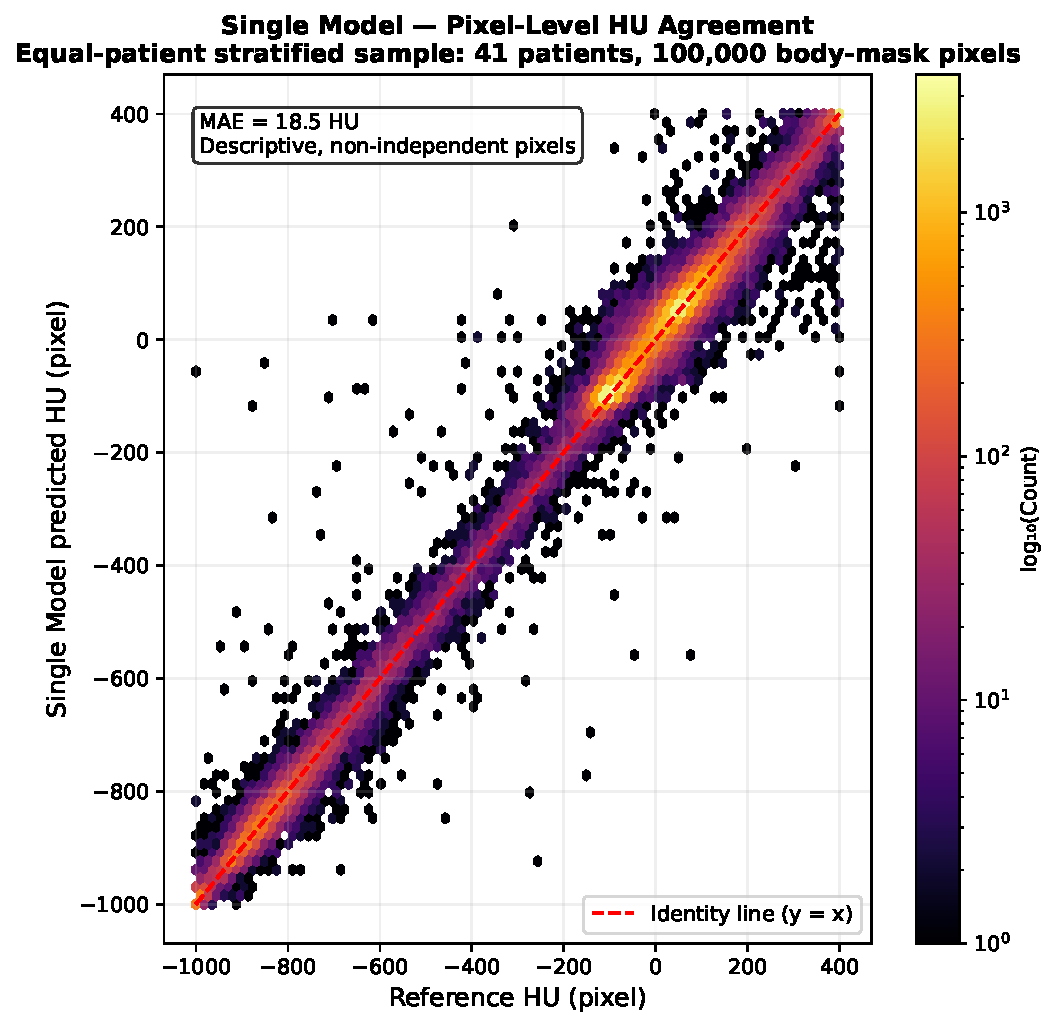
\includegraphics[width=0.82\linewidth]{Figures/Generated/evaluation_final/Appendix/scatter_pixel_hu_balanced.pdf}
    \captionsetup{skip=1.5pt}
    \graphiccaption[Pixel-level HU agreement]{Pixel-level HU agreement between the Single Model reconstruction and the clean reference. The hexbin uses a fixed equal-patient stratified sample of 100,000 valid body-mask pixels from 41 test-set patients. It is a descriptive calibration diagnostic. No hypothesis test or confidence interval is derived from the sampled pixels.}
    \label{fig:appendix-pixel-hu-agreement}
\end{figure}

The following plots complement the global-delta histograms presented in the main text. Each point represents one test slice, so these plots were not used for statistical inference.

\begingroup
\setlength{\intextsep}{4pt}
\begin{figure}[H]
    \centering
    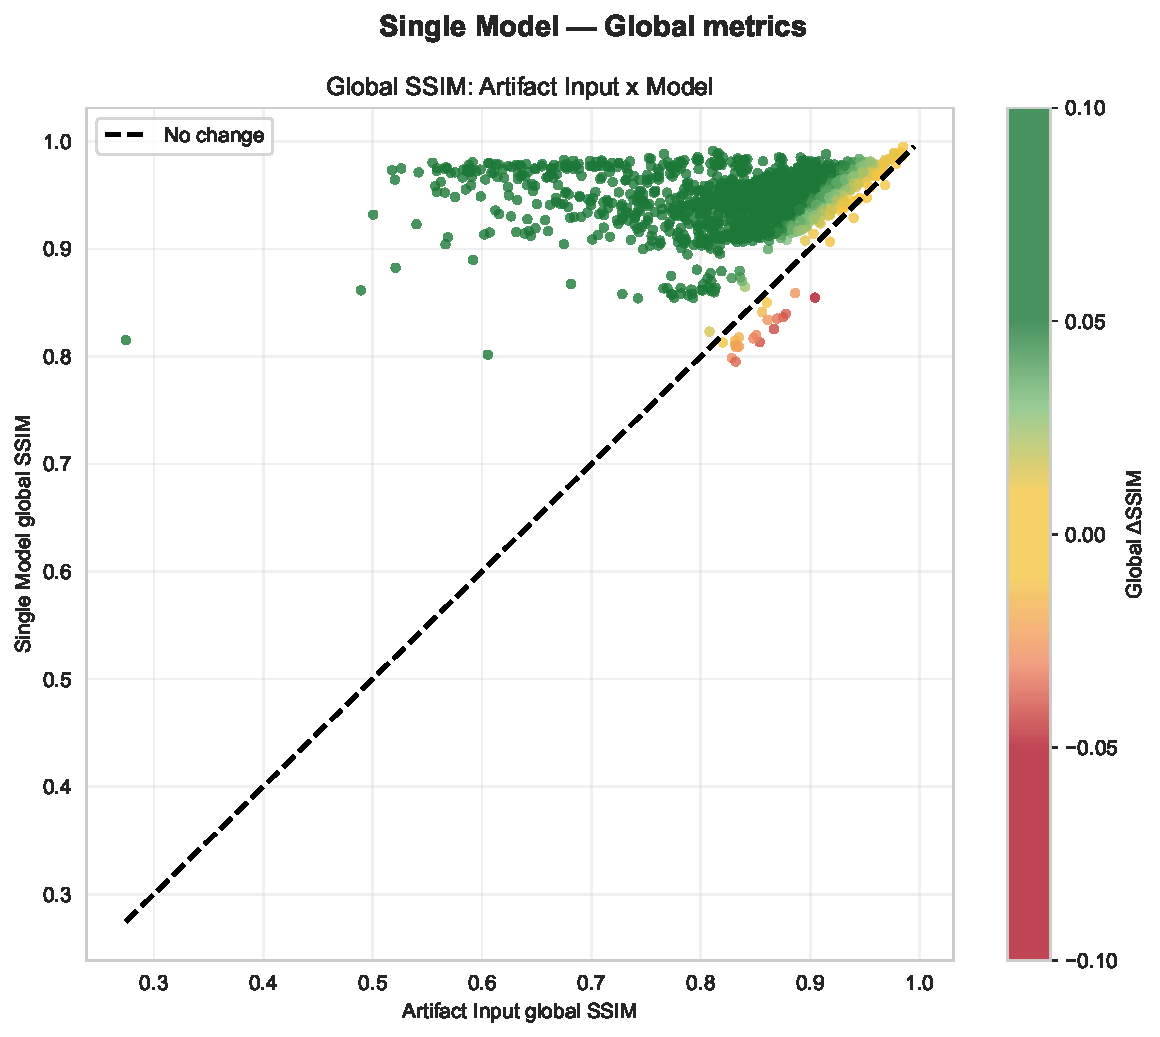
\includegraphics[width=0.84\linewidth]{Figures/Generated/evaluation_final/Appendix/scatter_global_ssim_baseline_vs_model.pdf}
\end{figure}

\begin{figure}[H]
    \centering
    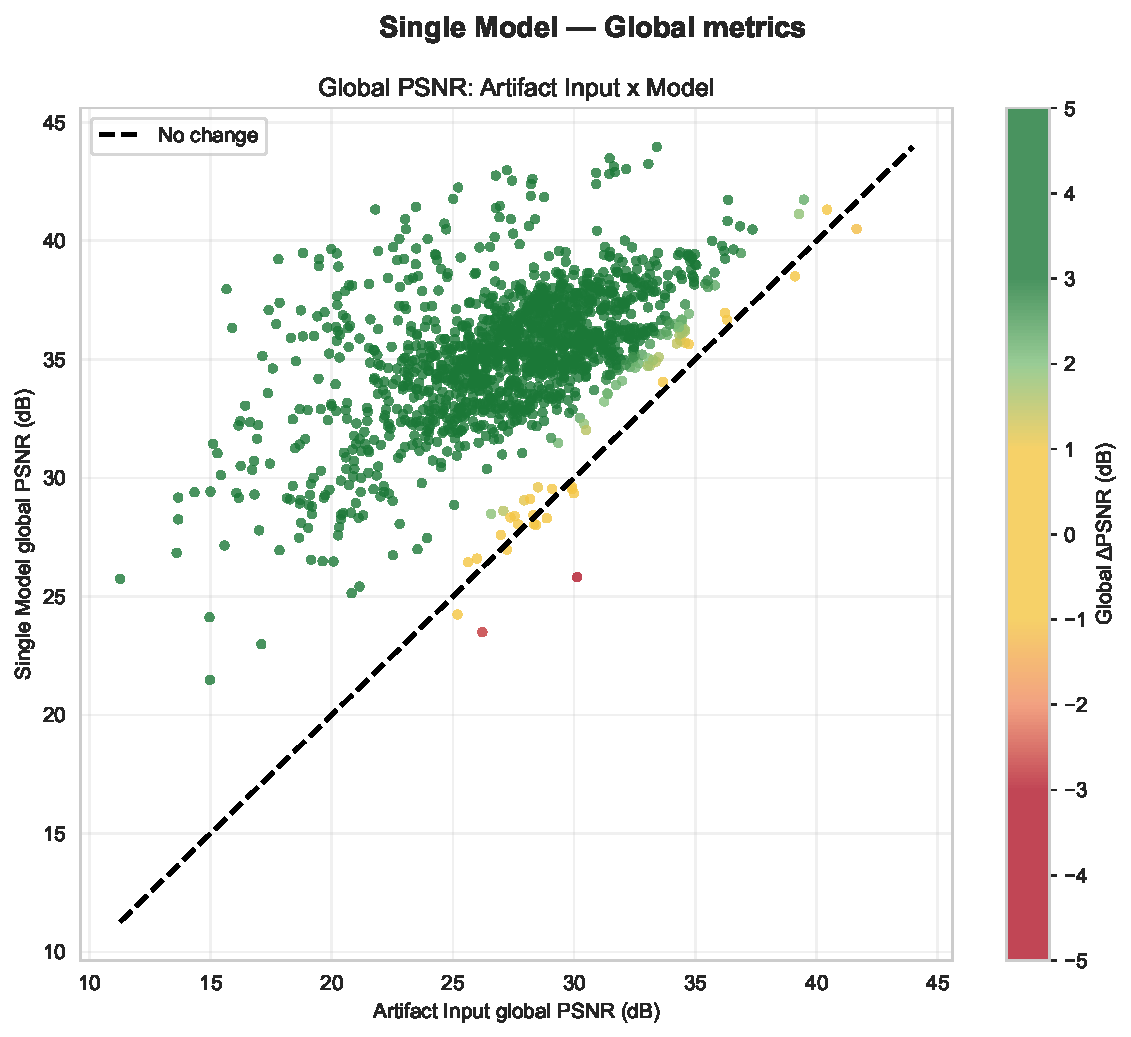
\includegraphics[width=0.84\linewidth]{Figures/Generated/evaluation_final/Appendix/scatter_global_psnr_baseline_vs_model.pdf}
\end{figure}
\captionsetup{skip=1.5pt}
\graphiccaptionof[Per-image input-output global metrics]{Per-image global SSIM (top) and PSNR (bottom) for the corrupted input and the Single Model reconstruction, seed 2024. The identity line denotes no change, marker color encodes the corresponding global delta. These slice-level relationships are descriptive, whereas statistical inference used patient-level aggregation.}
\label{fig:appendix-global-input-model}
\endgroup

As an exploratory analysis of heterogeneity, \autoref{fig:appendix-artifact-load-association} relates artifact burden to global improvement. Each point represents the mean across all slices of one patient ($n=41$), giving each patient equal weight. Artifact burden was defined as the mean artifact-area/body-area fraction per slice. Deltas correspond to the reconstruction metric minus the input metric, both calculated against the clean reference. Two-sided Spearman correlations were calculated with paired BCa bootstrap 95\% confidence intervals (10\,000 resamples; seed 1337), and the trend curve is a LOWESS estimate from \textit{Statsmodels}. This analysis was not part of the primary hypothesis-testing family and did not receive Holm adjustment. A positive association was observed between artifact burden and improvement: $\rho=0{.}479$ for $\Delta$PSNR (95\% CI [0{.}156; 0{.}717], $p=0{.}00154$) and $\rho=0{.}569$ for $\Delta$SSIM (95\% CI [0{.}225; 0{.}794], $p=0{.}000104$).

\begingroup
\setlength{\intextsep}{4pt}
\begin{figure}[H]
    \centering
    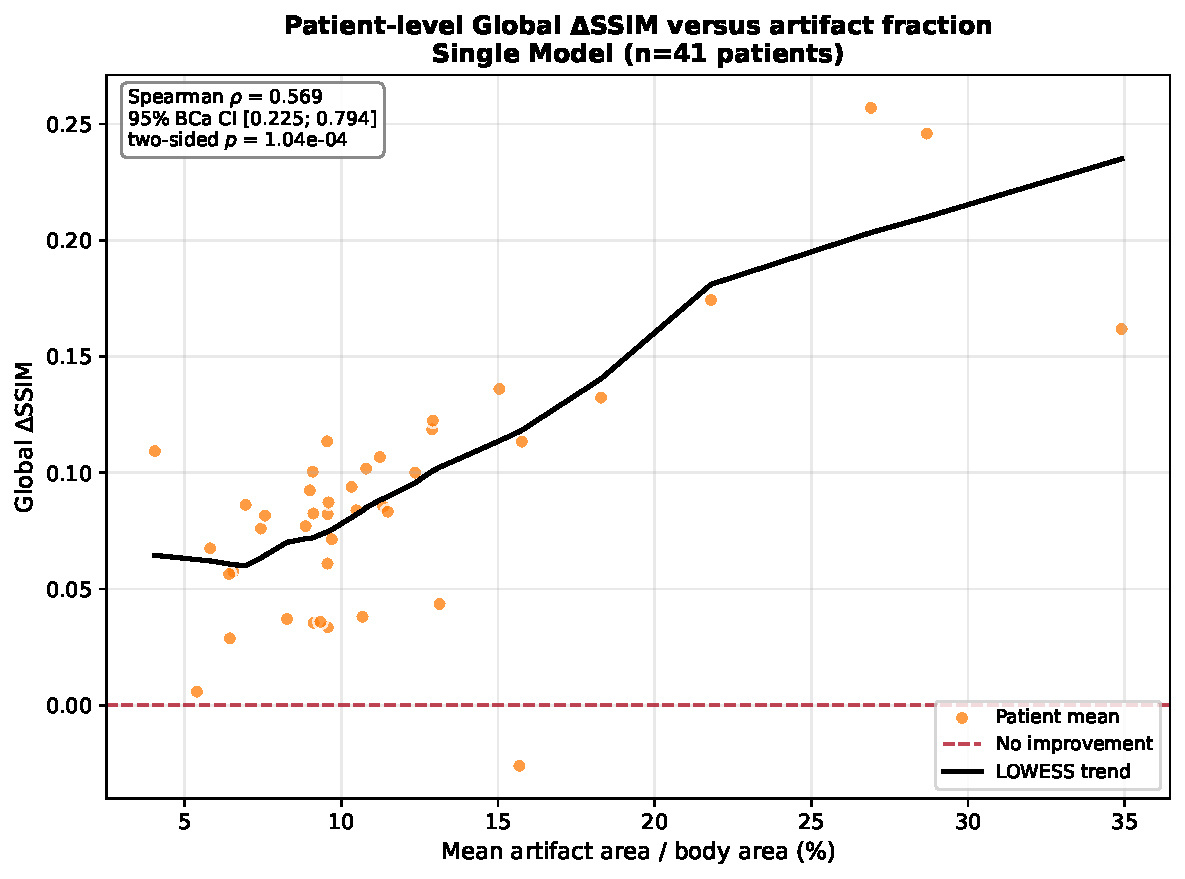
\includegraphics[width=0.84\linewidth]{Figures/Generated/evaluation_final/Appendix/scatter_patient_delta_ssim_vs_artifact_fraction_singlehead-033-0.9511-ssim_hu.pdf}
\end{figure}

\begin{figure}[H]
    \centering
    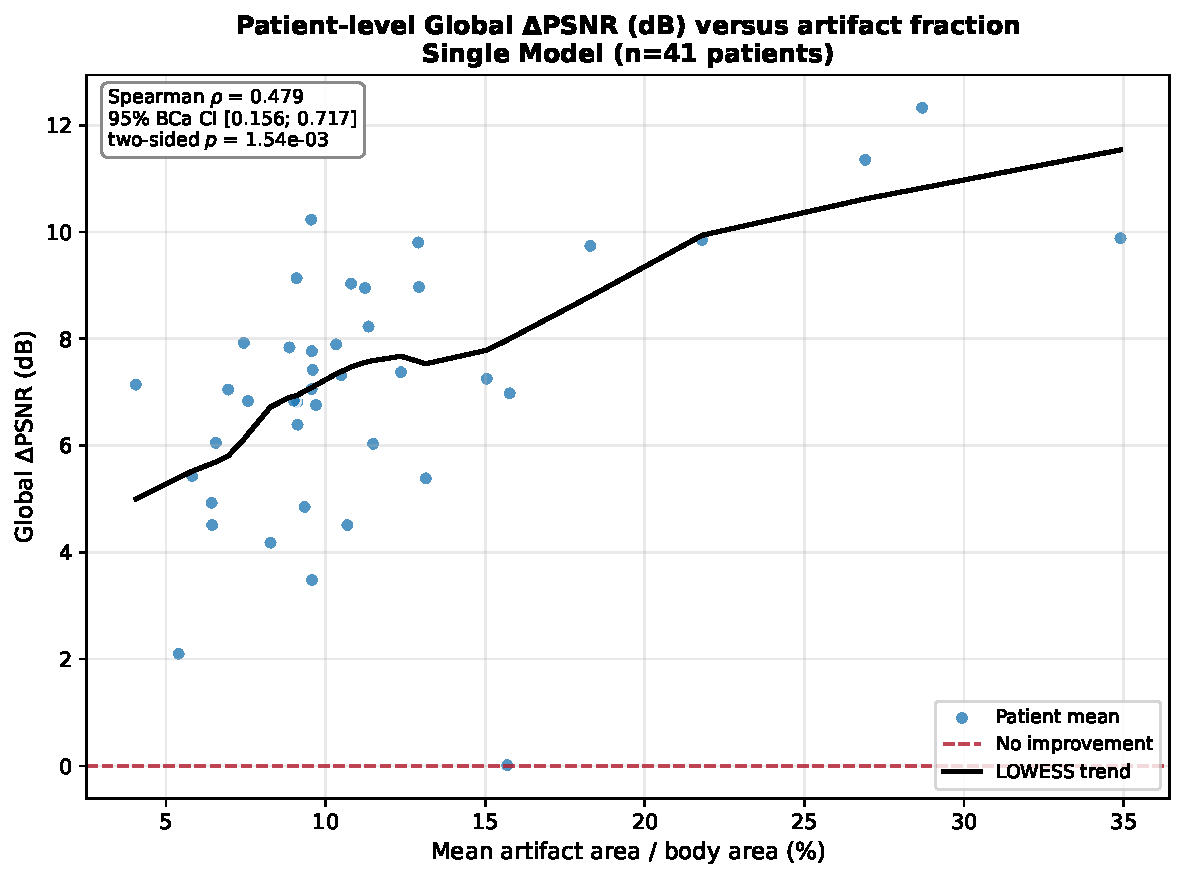
\includegraphics[width=0.84\linewidth]{Figures/Generated/evaluation_final/Appendix/scatter_patient_delta_psnr_vs_artifact_fraction_singlehead-033-0.9511-ssim_hu.pdf}
\end{figure}
\captionsetup{skip=1.5pt}
\graphiccaptionof[Patient-level artifact load and improvement]{Exploratory patient-level association between mean artifact fraction and global improvement for the Single Model, seed 2024: $\Delta$SSIM (top) and $\Delta$PSNR (bottom). Each point is one patient's mean across its test-set slices ($n=41$). Lines show Statsmodels LOWESS trends. Annotations report two-sided Spearman correlations and paired BCa bootstrap 95\% confidence intervals.}
\label{fig:appendix-artifact-load-association}
\endgroup

\section{Worst Performance Cases}
\label{sec:appendix-worst-cases}

As a complementary characterization of lower-performing slices, two slice-level groups were identified for the Single Model, seed 2024, in the test set: first by the bottom fifth percentile of global $\Delta$SSIM and then, complementarily, by the bottom fifth percentile of global $\Delta$PSNR. This slice-level classification is purely descriptive: it does not constitute a hypothesis test or reproduce the patient-level candidate-selection analysis, whose primary endpoint was Artifact-ROI $\Delta$SSIM, and it serves only to quantitatively situate the slice groups whose individual visual examples are discussed in \autoref{sec:residual-maps-extremes}.

Using the global $\Delta$SSIM criterion ($N=74$/1478 slices; threshold $=0{.}0146$), mean $\Delta$PSNR improvement remained positive ($1{.}88$~dB), but mean $\Delta$SSIM improvement was slightly negative ($-0{.}0019$). The mean Artifact-Zone\acrshort{mae} reduction was $65{.}2$~HU (\autoref{fig:appendix-worst-cases-ssim}). Thus, the most unfavorable subset according to this descriptive global criterion included a small mean\acrshort{ssim} degradation, even though most remaining slices continued to improve substantially.

\begin{figure}[H]
    \centering
    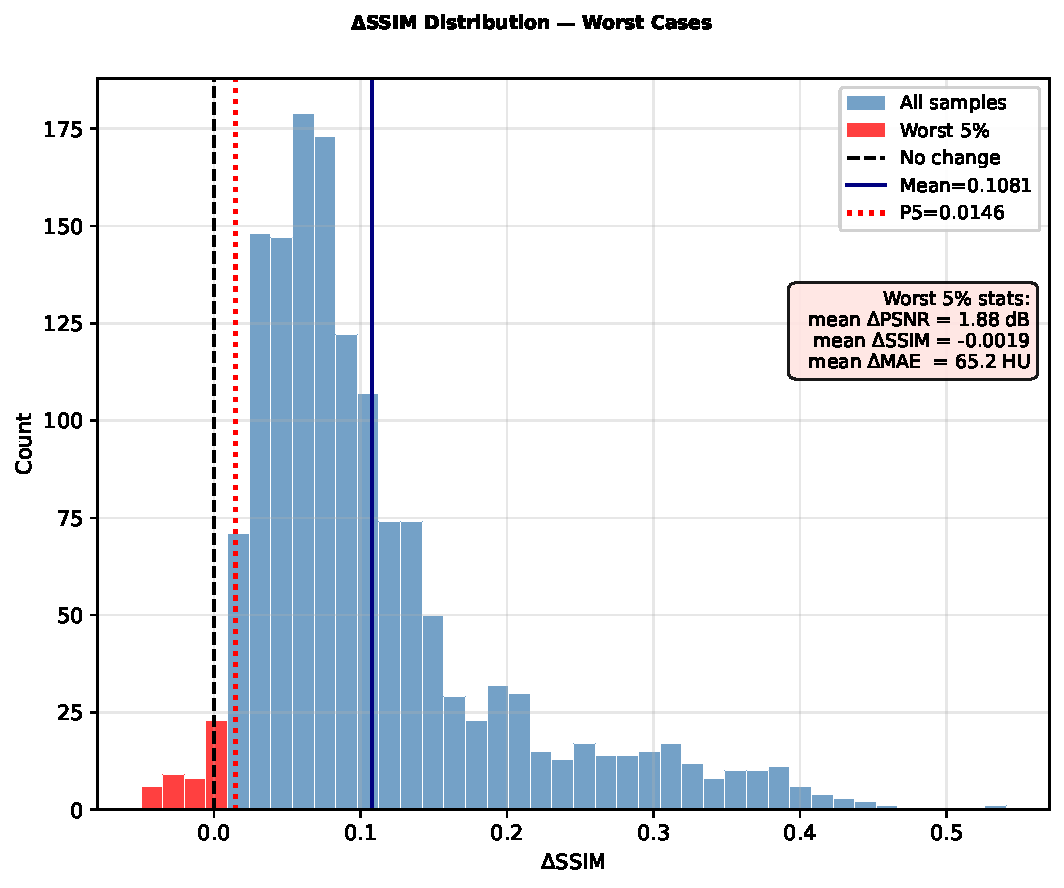
\includegraphics[width=0.84\linewidth]{Figures/Generated/evaluation_final/Appendix/worst_cases_ssim_distribution.pdf}
    \captionsetup{skip=1.5pt}
    \graphiccaption[Worst-case slices by global $\Delta$SSIM]{Bottom 5th-percentile slices by global $\Delta$SSIM for the Single Model, seed 2024, test split ($N=74$/1478, threshold $=0.0146$, highlighted in red). Descriptive. No inferential test is derived from this subset.}
    \label{fig:appendix-worst-cases-ssim}
\end{figure}

Using the complementary $\Delta$PSNR criterion ($N=74$/1478 slices; threshold $=2{.}59$~dB), this group was not identical to that defined by $\Delta$SSIM. Mean improvement remained positive for all three metrics (mean $\Delta$PSNR $=1{.}23$~dB, mean $\Delta$SSIM $=0{.}0071$, mean Artifact-Zone $\Delta$MAE $=62{.}0$~HU), although with substantial dispersion and some individual cases of degradation relative to the input, visible in the left tail of \autoref{fig:appendix-worst-cases-psnr}.

\begin{figure}[H]
    \centering
    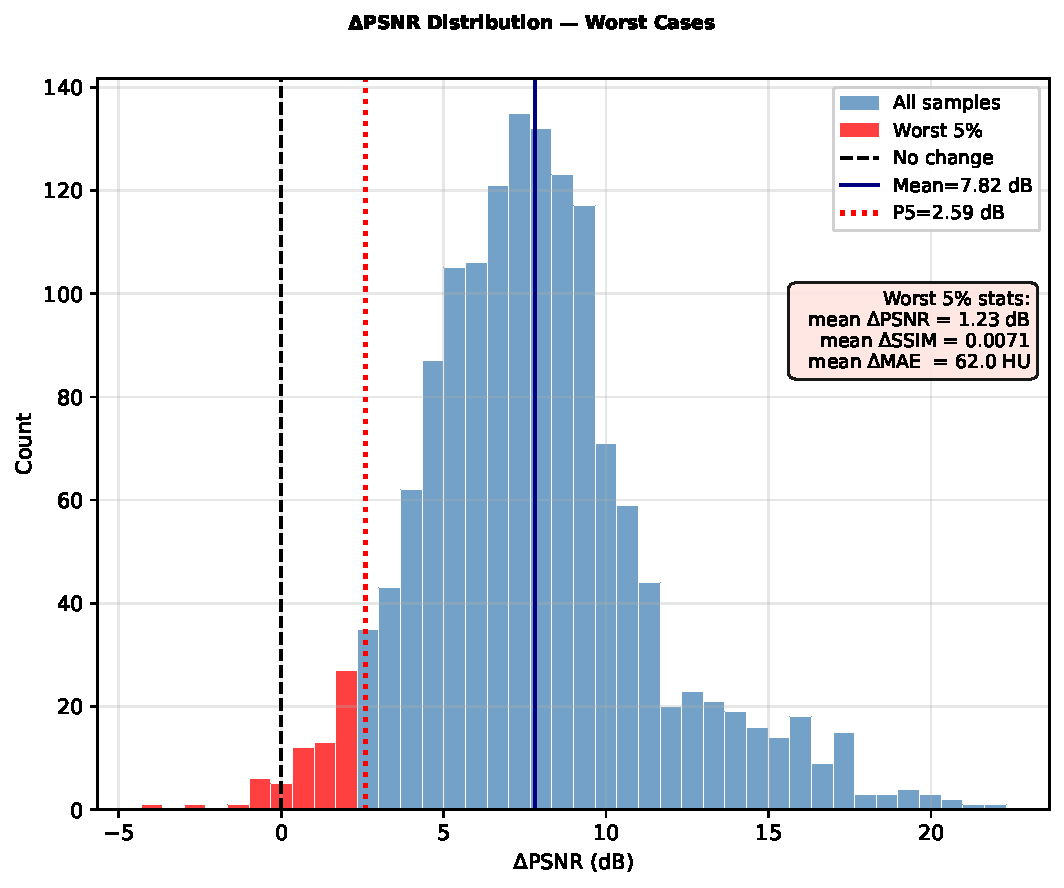
\includegraphics[width=0.84\linewidth]{Figures/Generated/evaluation_final/Appendix/worst_cases_delta_psnr_distribution.pdf}
    \captionsetup{skip=1.5pt}
    \graphiccaption[Worst-case slices by global $\Delta$PSNR]{Bottom 5th-percentile slices by global $\Delta$PSNR for the Single Model, seed 2024, test split ($N=74$/1478, threshold $=2.59$~dB, highlighted in red). Descriptive. No inferential test is derived from this subset.}
    \label{fig:appendix-worst-cases-psnr}
\end{figure}

Finally, \autoref{fig:appendix-worst-cases} jointly relates slice-level $\Delta$PSNR and $\Delta$SSIM, highlighting the lower-performance tail defined by $\Delta$PSNR in the preceding paragraph and allowing visualization of the bivariate dispersion of unfavorable cases.

\begin{figure}[H]
    \centering
    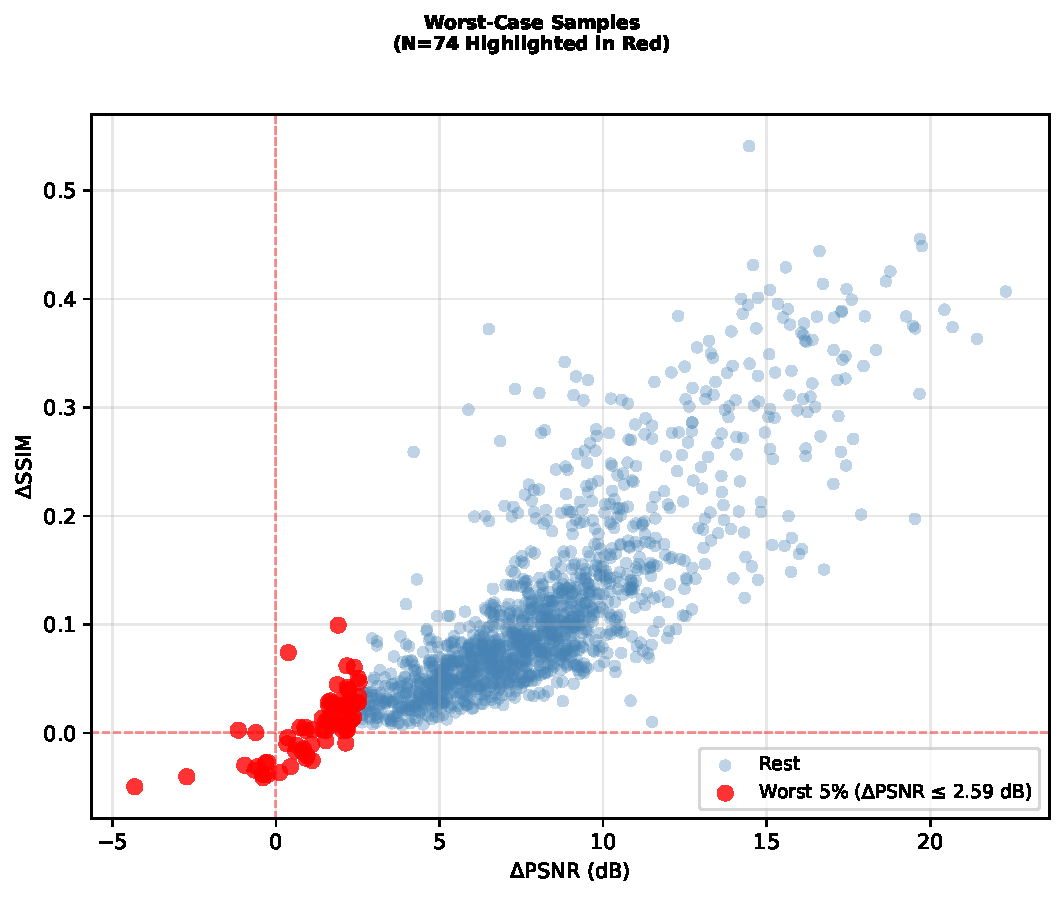
\includegraphics[width=0.84\linewidth]{Figures/Generated/evaluation_final/Appendix/worst_cases_scatter_delta_psnr_vs_delta_ssim.pdf}
    \captionsetup{skip=1.5pt}
    \graphiccaption[Worst-case slices: joint $\Delta$PSNR vs. $\Delta$SSIM]{Bottom 5th-percentile slices by global $\Delta$PSNR for the Single Model, seed 2024, test split ($N=74$/1478, threshold $=2.59$~dB, highlighted in red). $\Delta$PSNR vs. $\Delta$SSIM scatter. Descriptive. No inferential test is derived from this subset.}
    \label{fig:appendix-worst-cases}
\end{figure}

\section{Computational Performance}
\label{sec:appendix-computational-performance}

Runtime performance was quantified for the checkpoint of the model selected for external evaluation, on the internal test partition ($n=1478$ slices). The benchmark was run in the environment described in Materials and Methods, using an NVIDIA RTX A4500 GPU, batch size one, and five warm-up passes. For each slice, latency was measured from the model call to explicit synchronization of the output with the CPU. Consequently, this measurement includes inference execution and output synchronization, but excludes image loading and external preprocessing or result-presentation stages.

Mean latency was $24{.}13\,\mathrm{ms}$ per slice (standard deviation: $0{.}69\,\mathrm{ms}$, median: $24{.}30\,\mathrm{ms}$), corresponding to a throughput of $41{.}4$ slices per second. The 95th and 99th percentiles were $24{.}66\,\mathrm{ms}$ and $27{.}53\,\mathrm{ms}$ per slice, respectively. The proximity of the mean, median, and 95th percentile indicates latency stability for most runs. The complete distribution and slice-level variation are shown in \autoref{fig:benchmark-latency}. These values characterize the experimental configuration used and do not, by themselves, represent the response time of a complete clinical workflow or of another computational environment.
% Generated by scripts/publish_workflow_results_to_thesis.py. Do not edit.
\begingroup
\setlength{\intextsep}{4pt}
\begin{figure}[H]
    \centering
    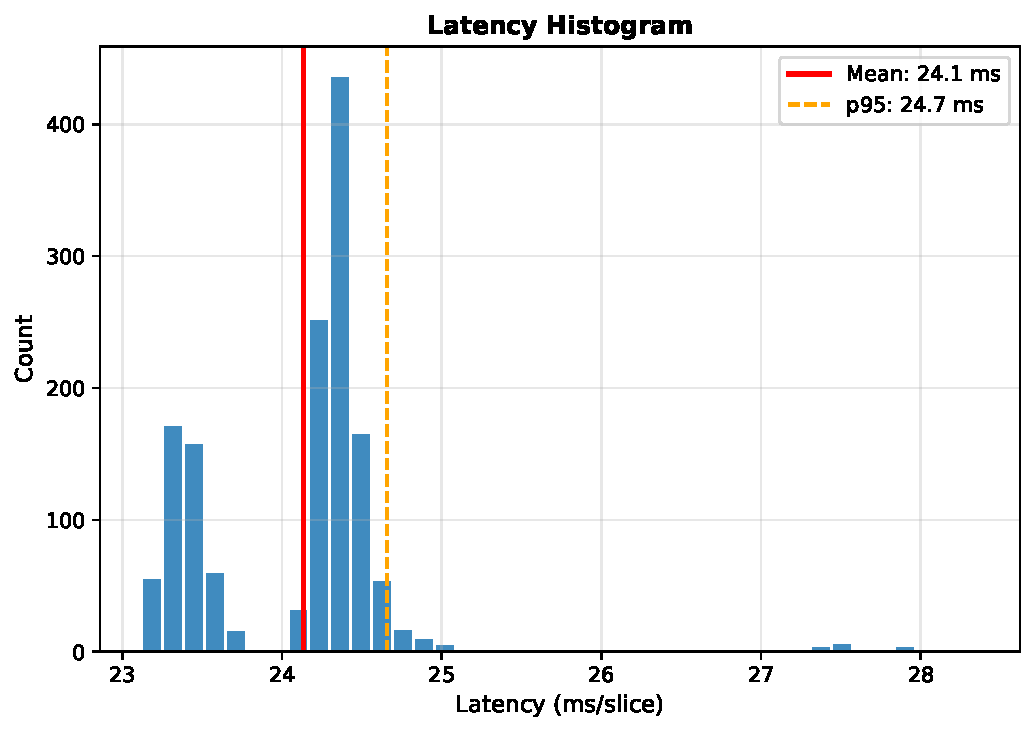
\includegraphics[width=0.84\linewidth]{Figures/Generated/benchmark/benchmark-latency-histogram-91086c81.pdf}
\end{figure}

\begin{figure}[H]
    \centering
    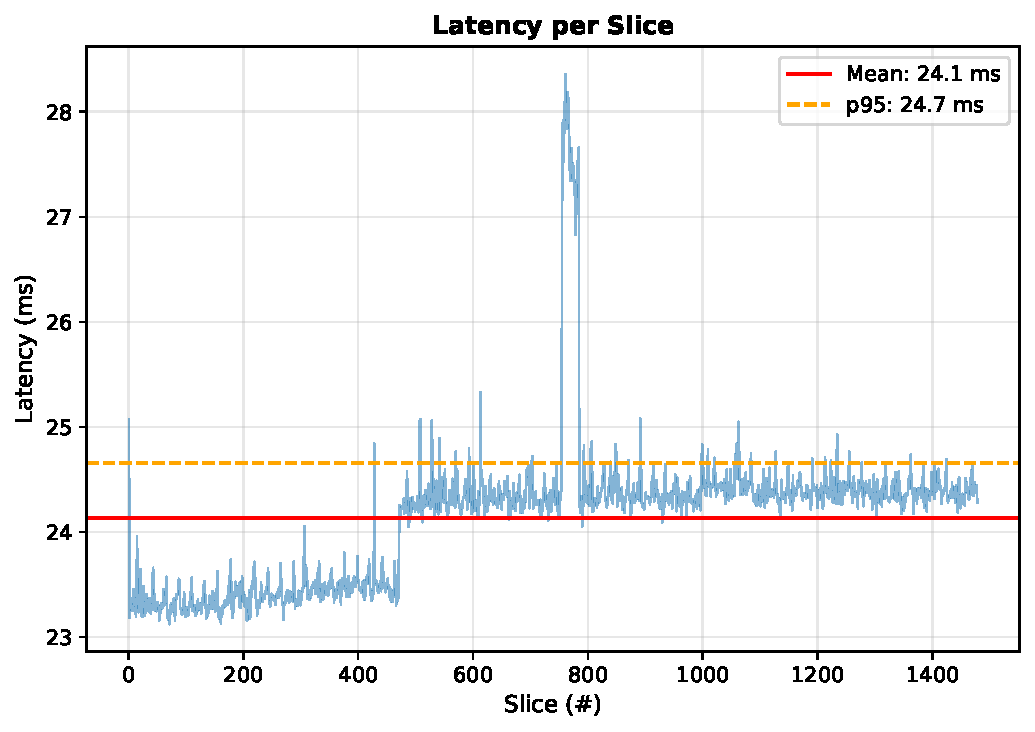
\includegraphics[width=0.84\linewidth]{Figures/Generated/benchmark/benchmark-latency-per-slice-fe3b1d76.pdf}
\end{figure}

\captionsetup{skip=1.5pt}
\graphiccaptionof[Benchmark Latency]{Inference benchmark: latency histogram and latency per slice.}
\label{fig:benchmark-latency}
\endgroup

